\section{Dataset Samples}

\subsection{TB Chest X-ray Dataset Sample}

\textbf{Source:} National Institutes of Health (NIH) Chest X-ray Database, Kaggle Public Repository

\textbf{Total Images:} 7,000 \\
\textbf{Classes:} Normal (3,500), TB Positive (3,500)

\textbf{Image Specifications:}
\begin{itemize}
    \item Format: JPEG, Grayscale
    \item Resolution: 512$\times$512 to 1024$\times$1024 pixels
    \item Bit Depth: 8-bit (256 gray levels)
    \item File Size: 50-200 KB per image
\end{itemize}

\textbf{Distribution Across Hospitals:}
\begin{itemize}
    \item \textbf{Hospital 1:} 3,500 images (70\% TB positive—diagnostic center specializing in TB cases)
    \item \textbf{Hospital 2:} 3,500 images (30\% TB positive—general screening population)
\end{itemize}

\textbf{Sample Characteristics:}
\begin{itemize}
    \item TB-positive images show cavitary lesions, infiltrates, pleural effusion
    \item Normal images show clear lung fields, normal cardiac silhouette
    \item Variations in patient positioning (frontal, slight rotation)
    \item Equipment differences reflected in contrast and resolution
\end{itemize}

\subsection{Diabetic Retinopathy Dataset Sample}

\textbf{Source:} Kaggle Diabetic Retinopathy Detection Competition, EyePACS Dataset

\textbf{Total Images:} 3,662 \\
\textbf{Classes:} 0-No DR (1,831), 1-Mild (549), 2-Moderate (732), 3-Severe (366), 4-Proliferative (184)

\textbf{Image Specifications:}
\begin{itemize}
    \item Format: JPEG, RGB Color
    \item Resolution: 2048$\times$1536 to 4752$\times$3168 pixels
    \item Bit Depth: 24-bit color
    \item File Size: 200-800 KB per image
\end{itemize}

\textbf{Distribution Across Hospitals:}
\begin{itemize}
    \item \textbf{Hospital 1:} 1,831 images (tertiary care center—60\% severe cases, levels 3-4)
    \item \textbf{Hospital 2:} 1,831 images (screening population—75\% mild or no DR, levels 0-1)
\end{itemize}

\textbf{Sample Characteristics:}
\begin{itemize}
    \item Level 0: No visible abnormalities
    \item Level 1: Microaneurysms only
    \item Level 2: More than microaneurysms, less than severe
    \item Level 3: Hemorrhages, microaneurysms in 4 quadrants
    \item Level 4: Neovascularization, vitreous hemorrhage
\end{itemize}

\subsection{Brain Tumor MRI Dataset Sample}

\textbf{Source:} Kaggle Brain MRI Images, Harvard Medical School Dataset

\textbf{Total Images:} 3,624 \\
\textbf{Classes:} Glioma (906), Meningioma (937), Pituitary (901), No Tumor (880)

\textbf{Image Specifications:}
\begin{itemize}
    \item Format: JPEG, Grayscale
    \item Resolution: 512$\times$512 pixels
    \item Bit Depth: 8-bit
    \item File Size: 30-100 KB per image
    \item Modality: T1-weighted contrast-enhanced MRI
\end{itemize}

\textbf{Distribution Across Hospitals:}
\begin{itemize}
    \item \textbf{Hospital 1:} 1,812 images (neurosurgery center—50\% glioma cases)
    \item \textbf{Hospital 2:} 1,812 images (general neurology—balanced distribution across all tumor types)
\end{itemize}

\textbf{Sample Characteristics:}
\begin{itemize}
    \item Glioma: Irregular borders, heterogeneous enhancement
    \item Meningioma: Well-defined borders, homogeneous enhancement
    \item Pituitary: Central location, sellar region involvement
    \item No Tumor: Normal brain anatomy, no masses
\end{itemize}

\section{Application Screenshots}

This section presents the user interface and administrative dashboards of the Federated Learning platform.

\begin{figure}[H]
    \centering
    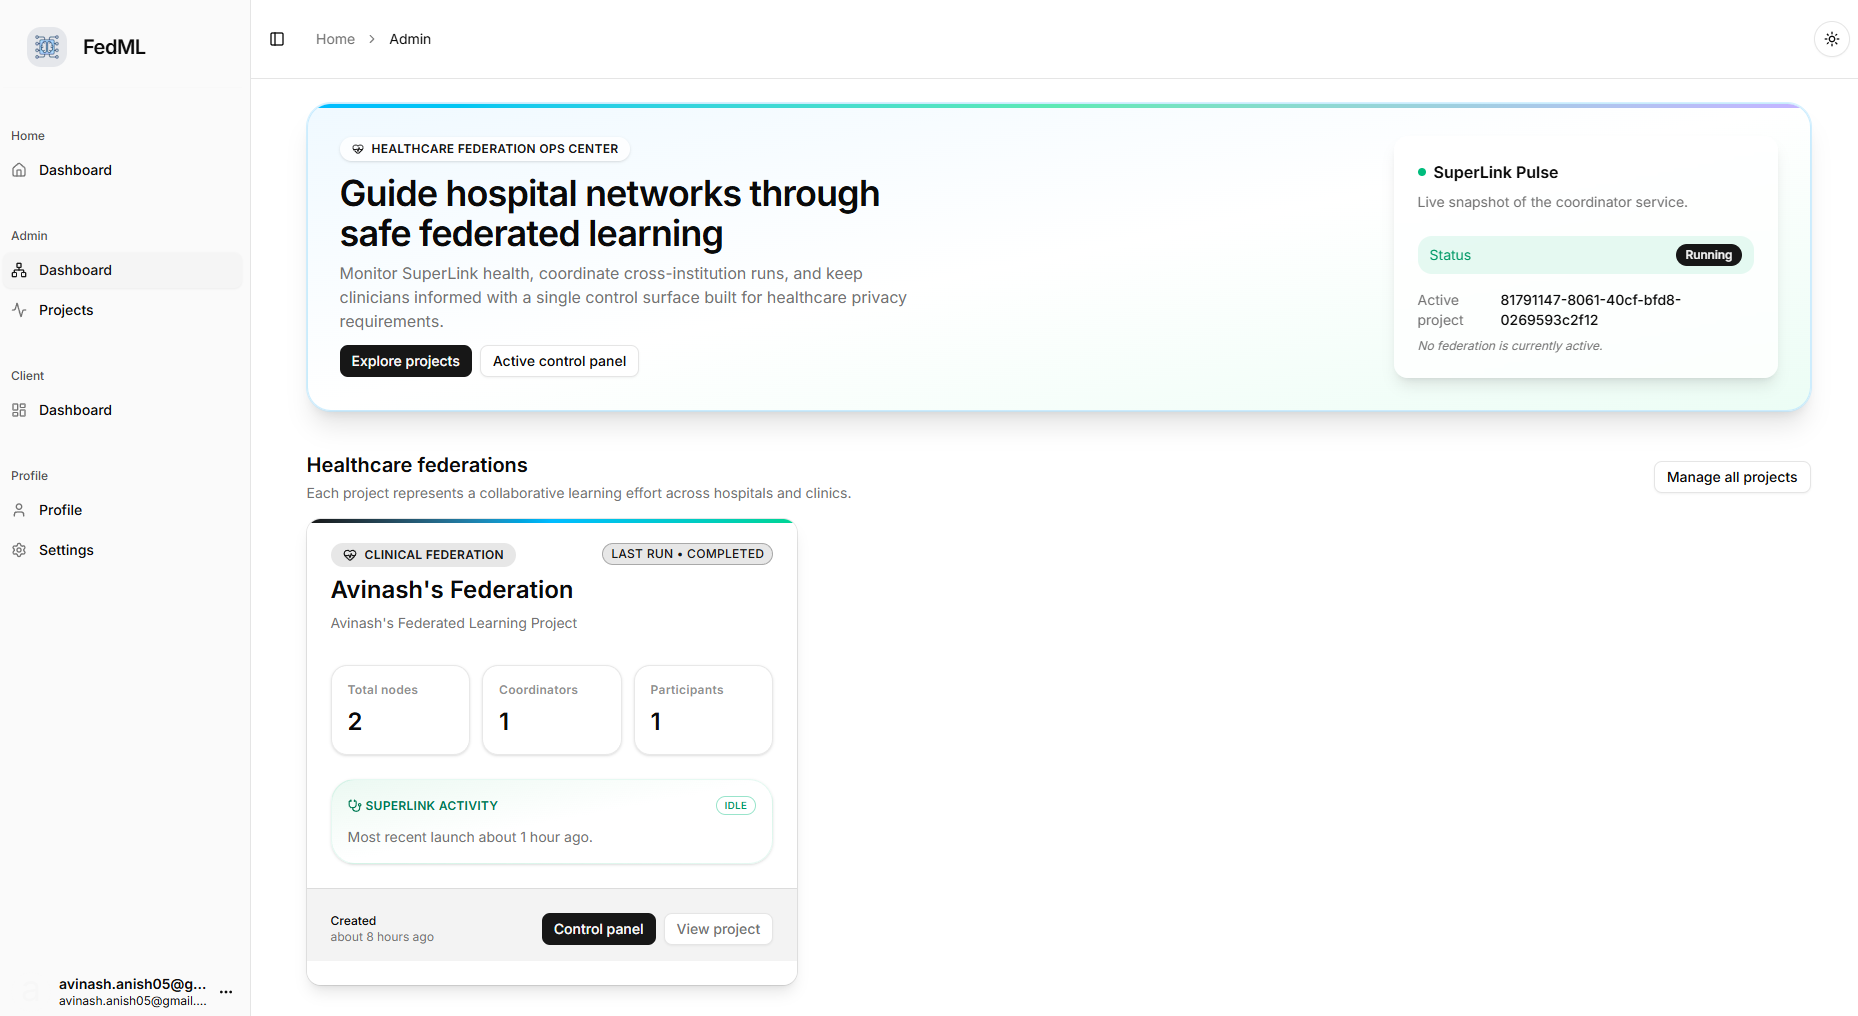
\includegraphics[width=0.9\textwidth]{images/screenshots/fedml-admin-dash.png}
    \caption{Administrator Dashboard providing an overview of training progress and system health.}
    \label{fig:admin_dash}
\end{figure}

\begin{figure}[H]
    \centering
    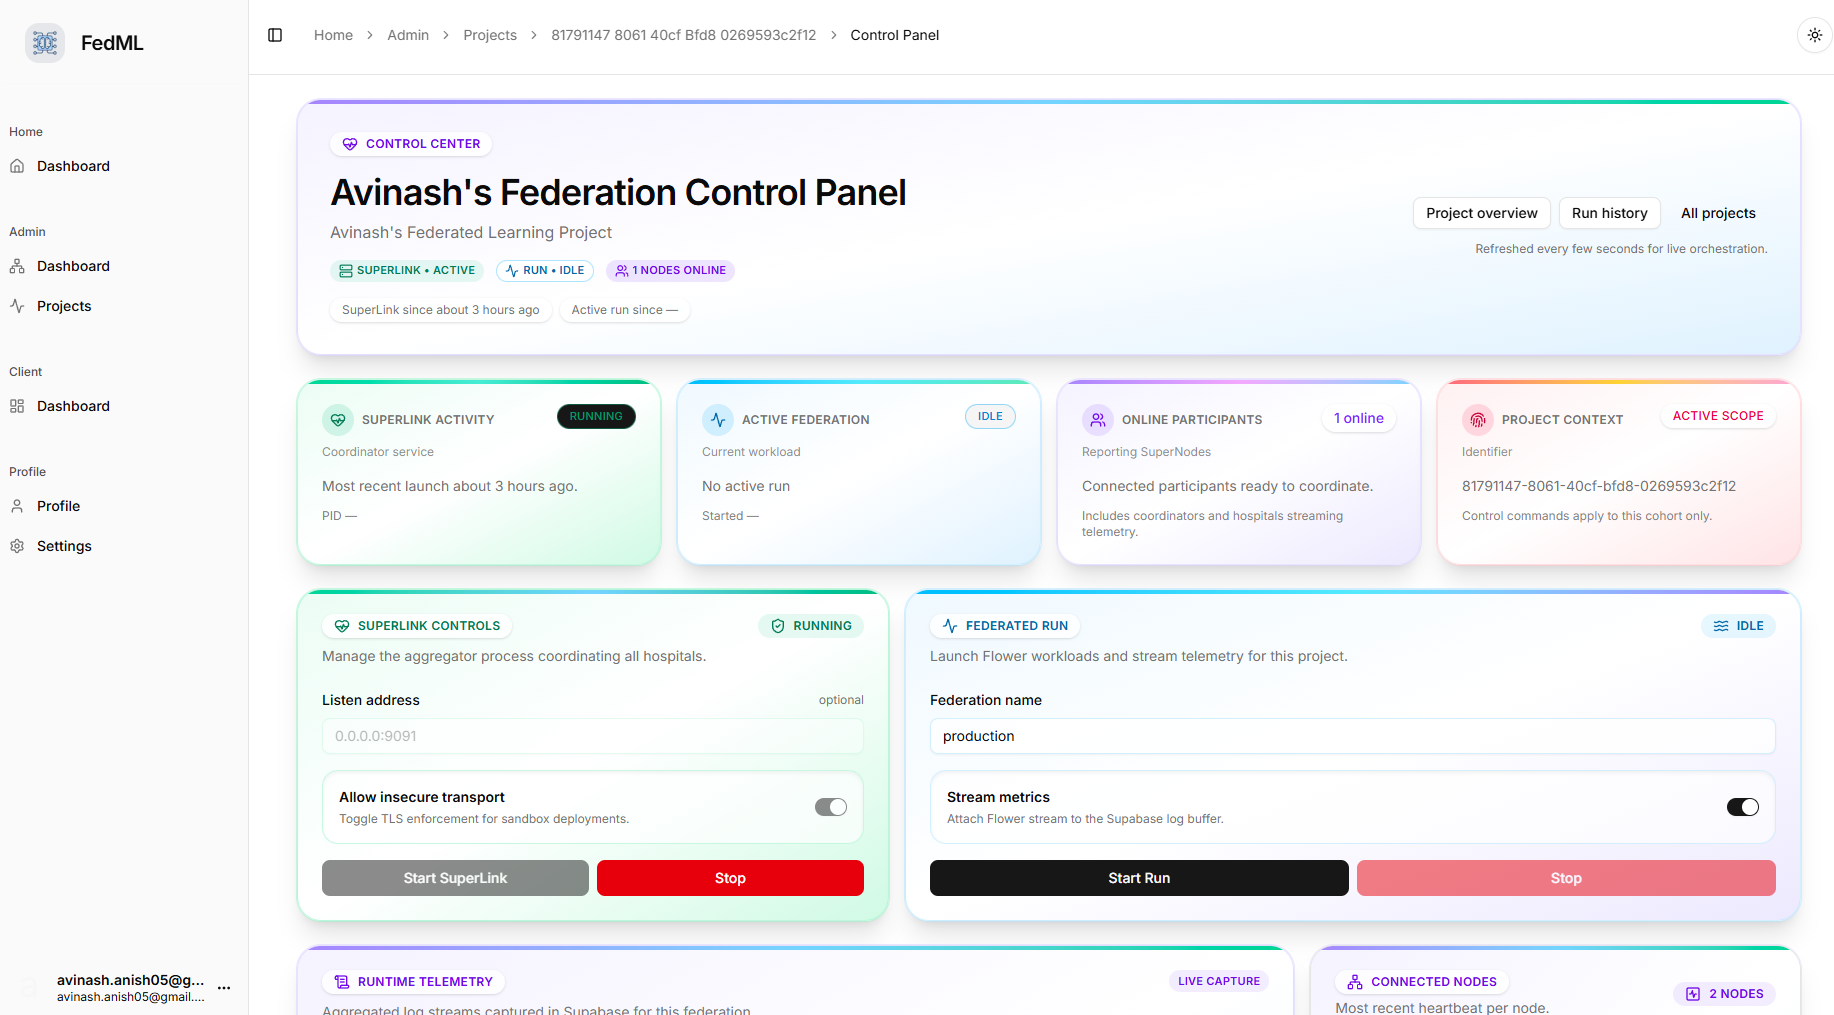
\includegraphics[width=0.9\textwidth]{images/screenshots/fedml-admin-control-panel.png}
    \caption{Admin Control Panel for managing federated runs and hospital institutions.}
    \label{fig:admin_control}
\end{figure}

\begin{figure}[H]
    \centering
    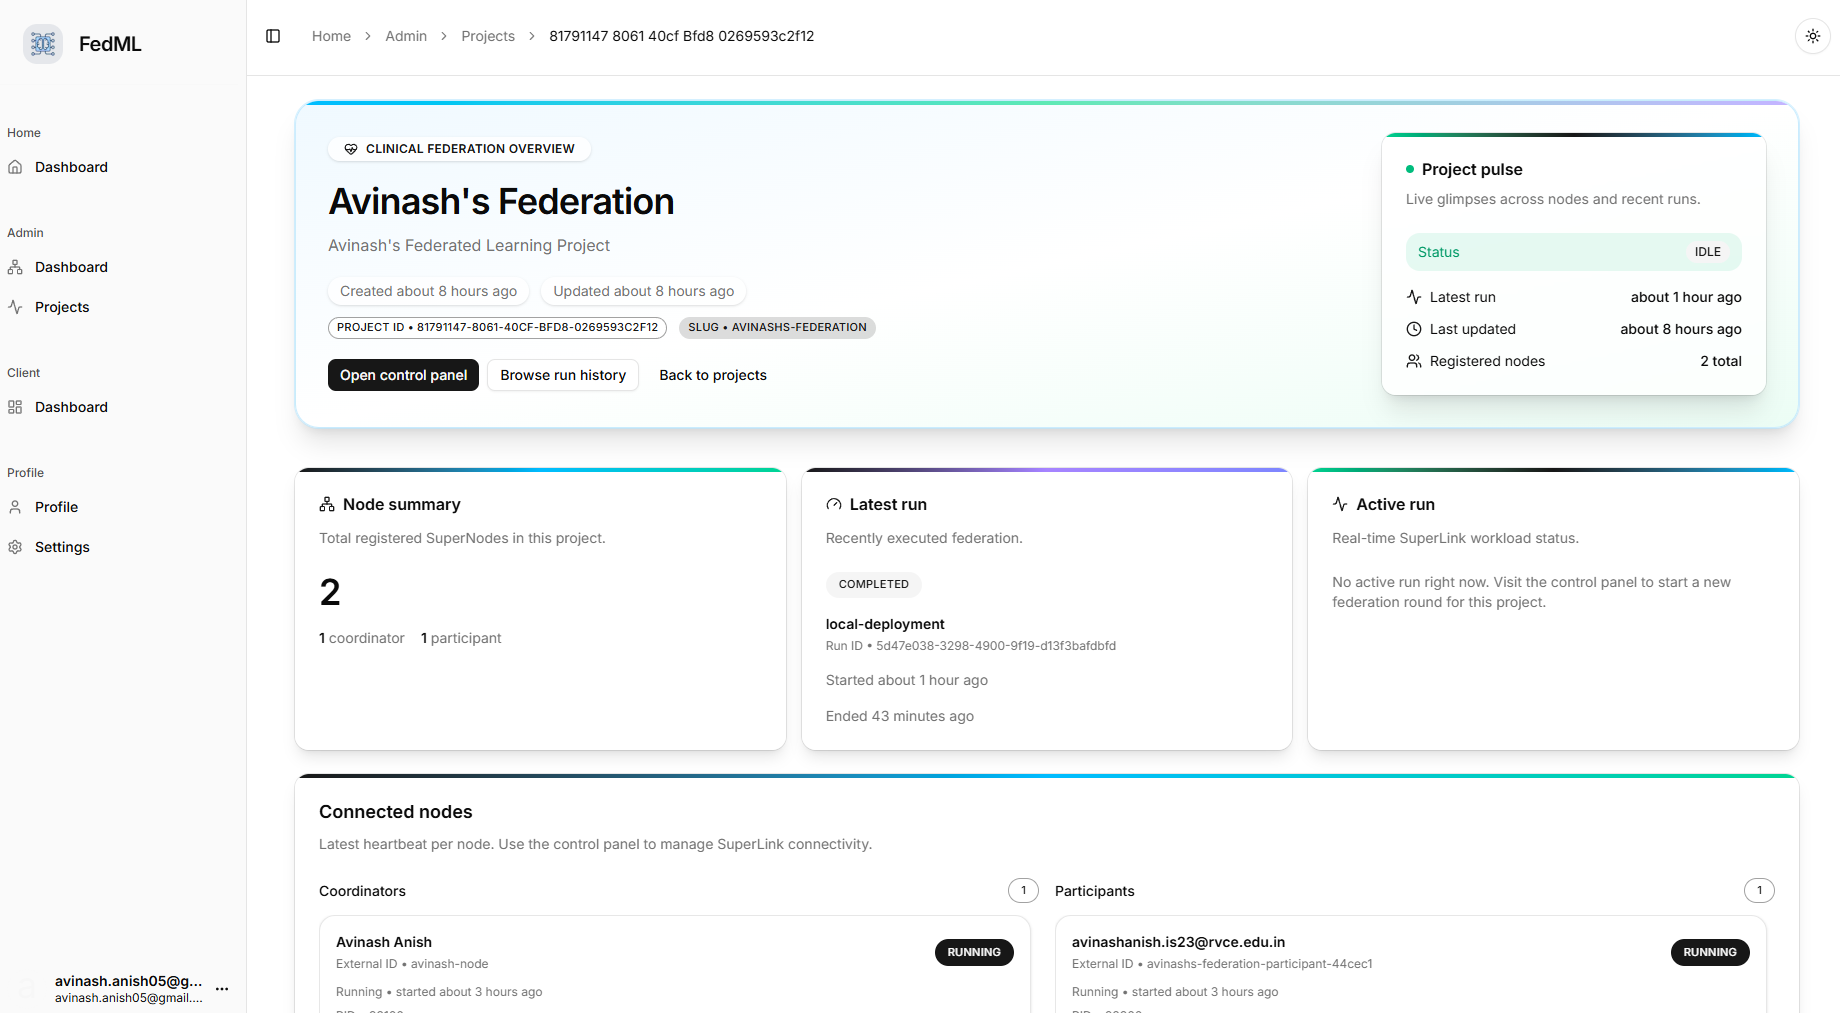
\includegraphics[width=0.9\textwidth]{images/screenshots/fedml-admin-project-details.png}
    \caption{Project Details view showing model configuration and dataset parameters.}
    \label{fig:project_details}
\end{figure}

\begin{figure}[H]
    \centering
    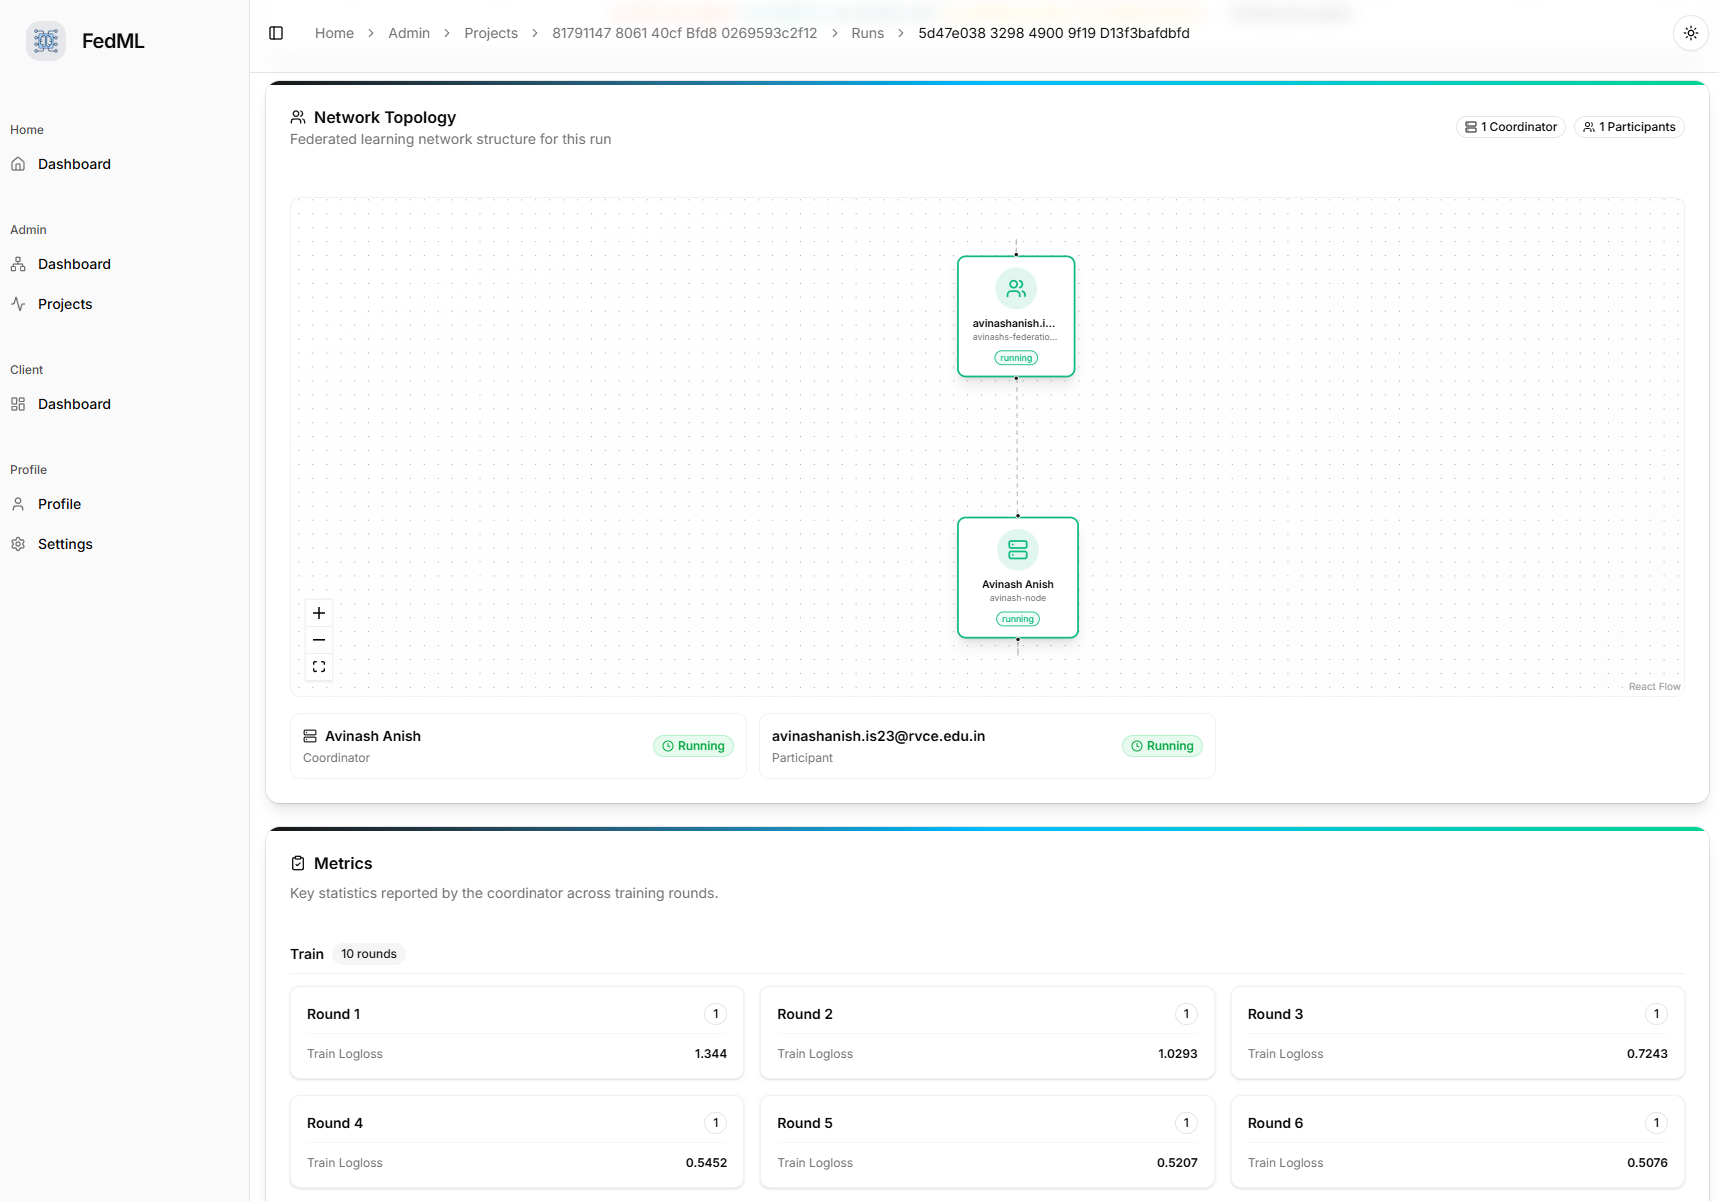
\includegraphics[width=0.9\textwidth]{images/screenshots/fedml-admin-project-details-topology.png}
    \caption{Network Topology visualization showing participating hospitals and central coordinator.}
    \label{fig:topology}
\end{figure}

\begin{figure}[H]
    \centering
    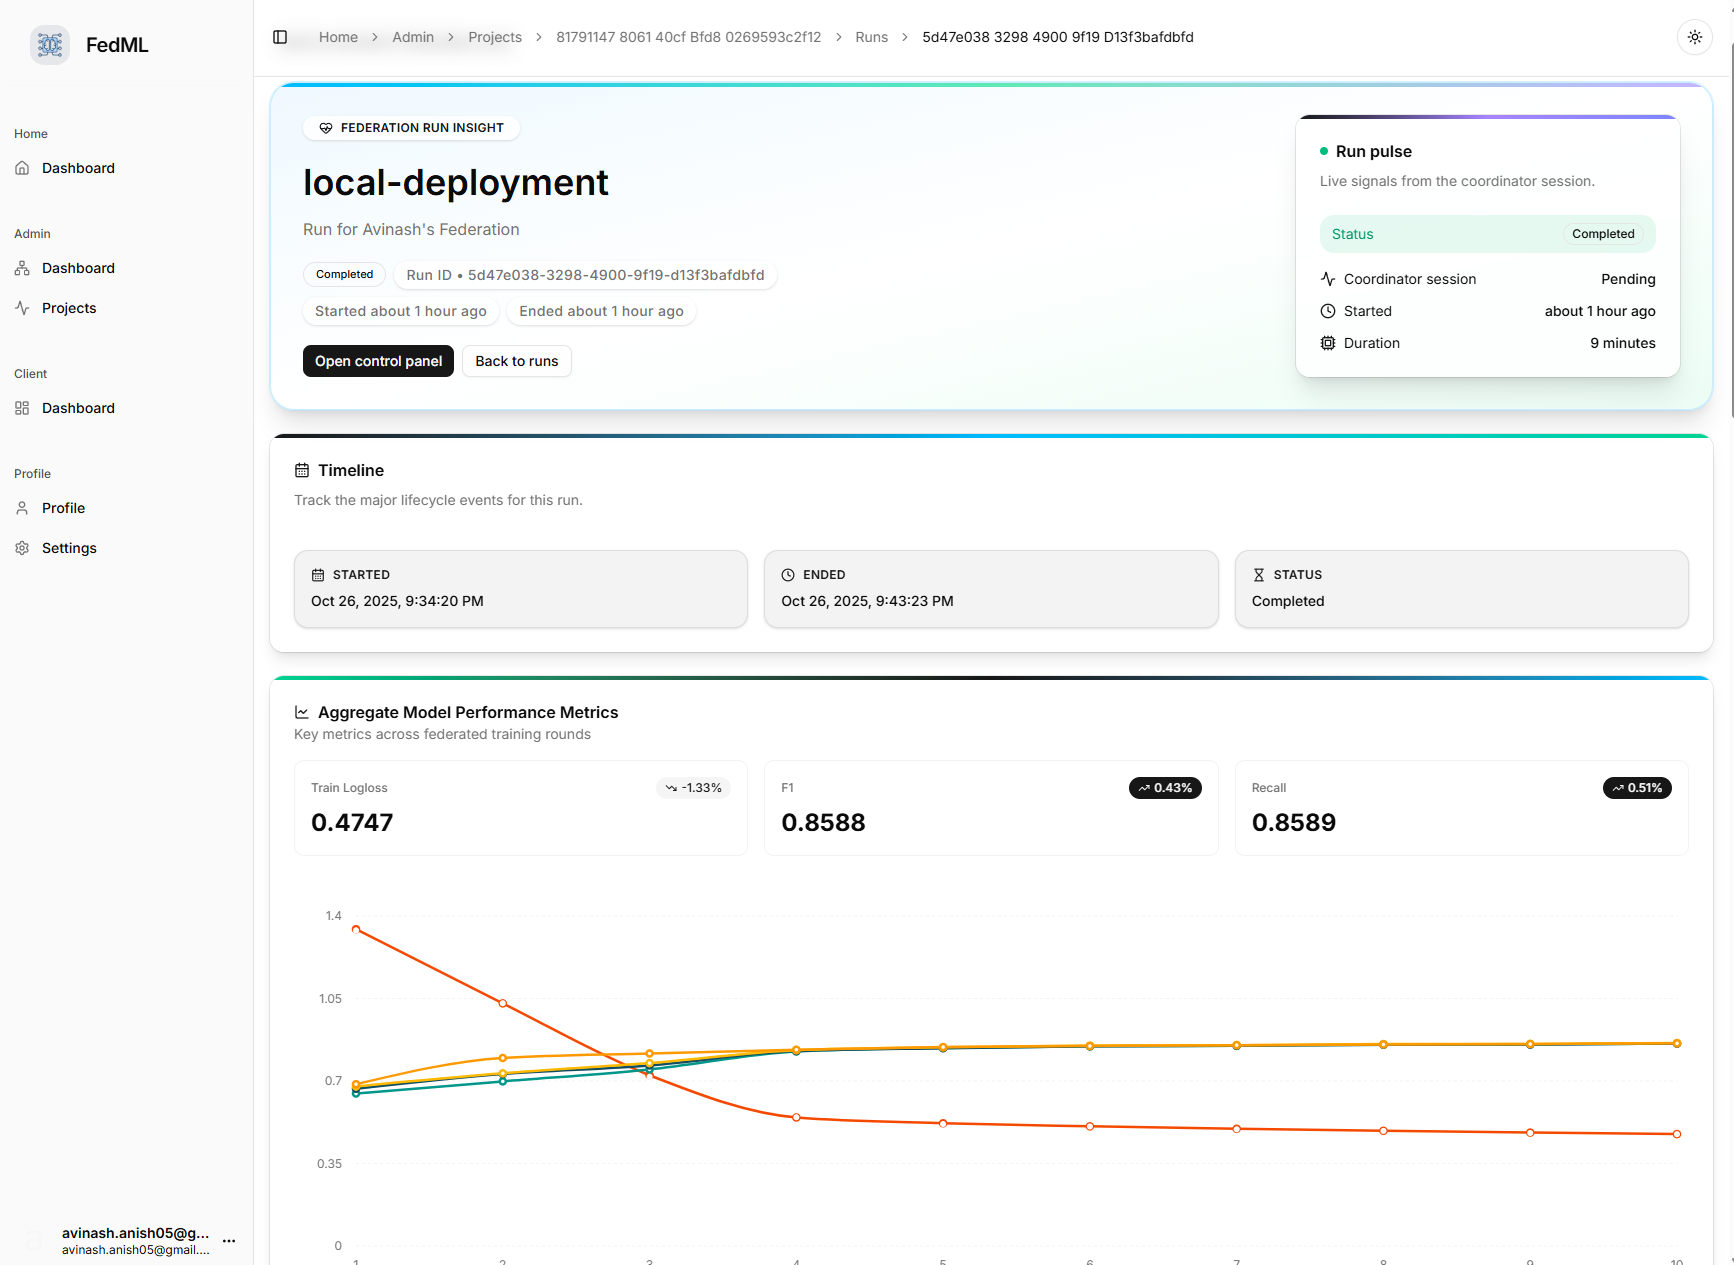
\includegraphics[width=0.9\textwidth]{images/screenshots/fedml-admin-run-details.png}
    \caption{Real-time training metrics for a specific federated round showing accuracy/loss curves.}
    \label{fig:run_details}
\end{figure}

\begin{figure}[H]
    \centering
    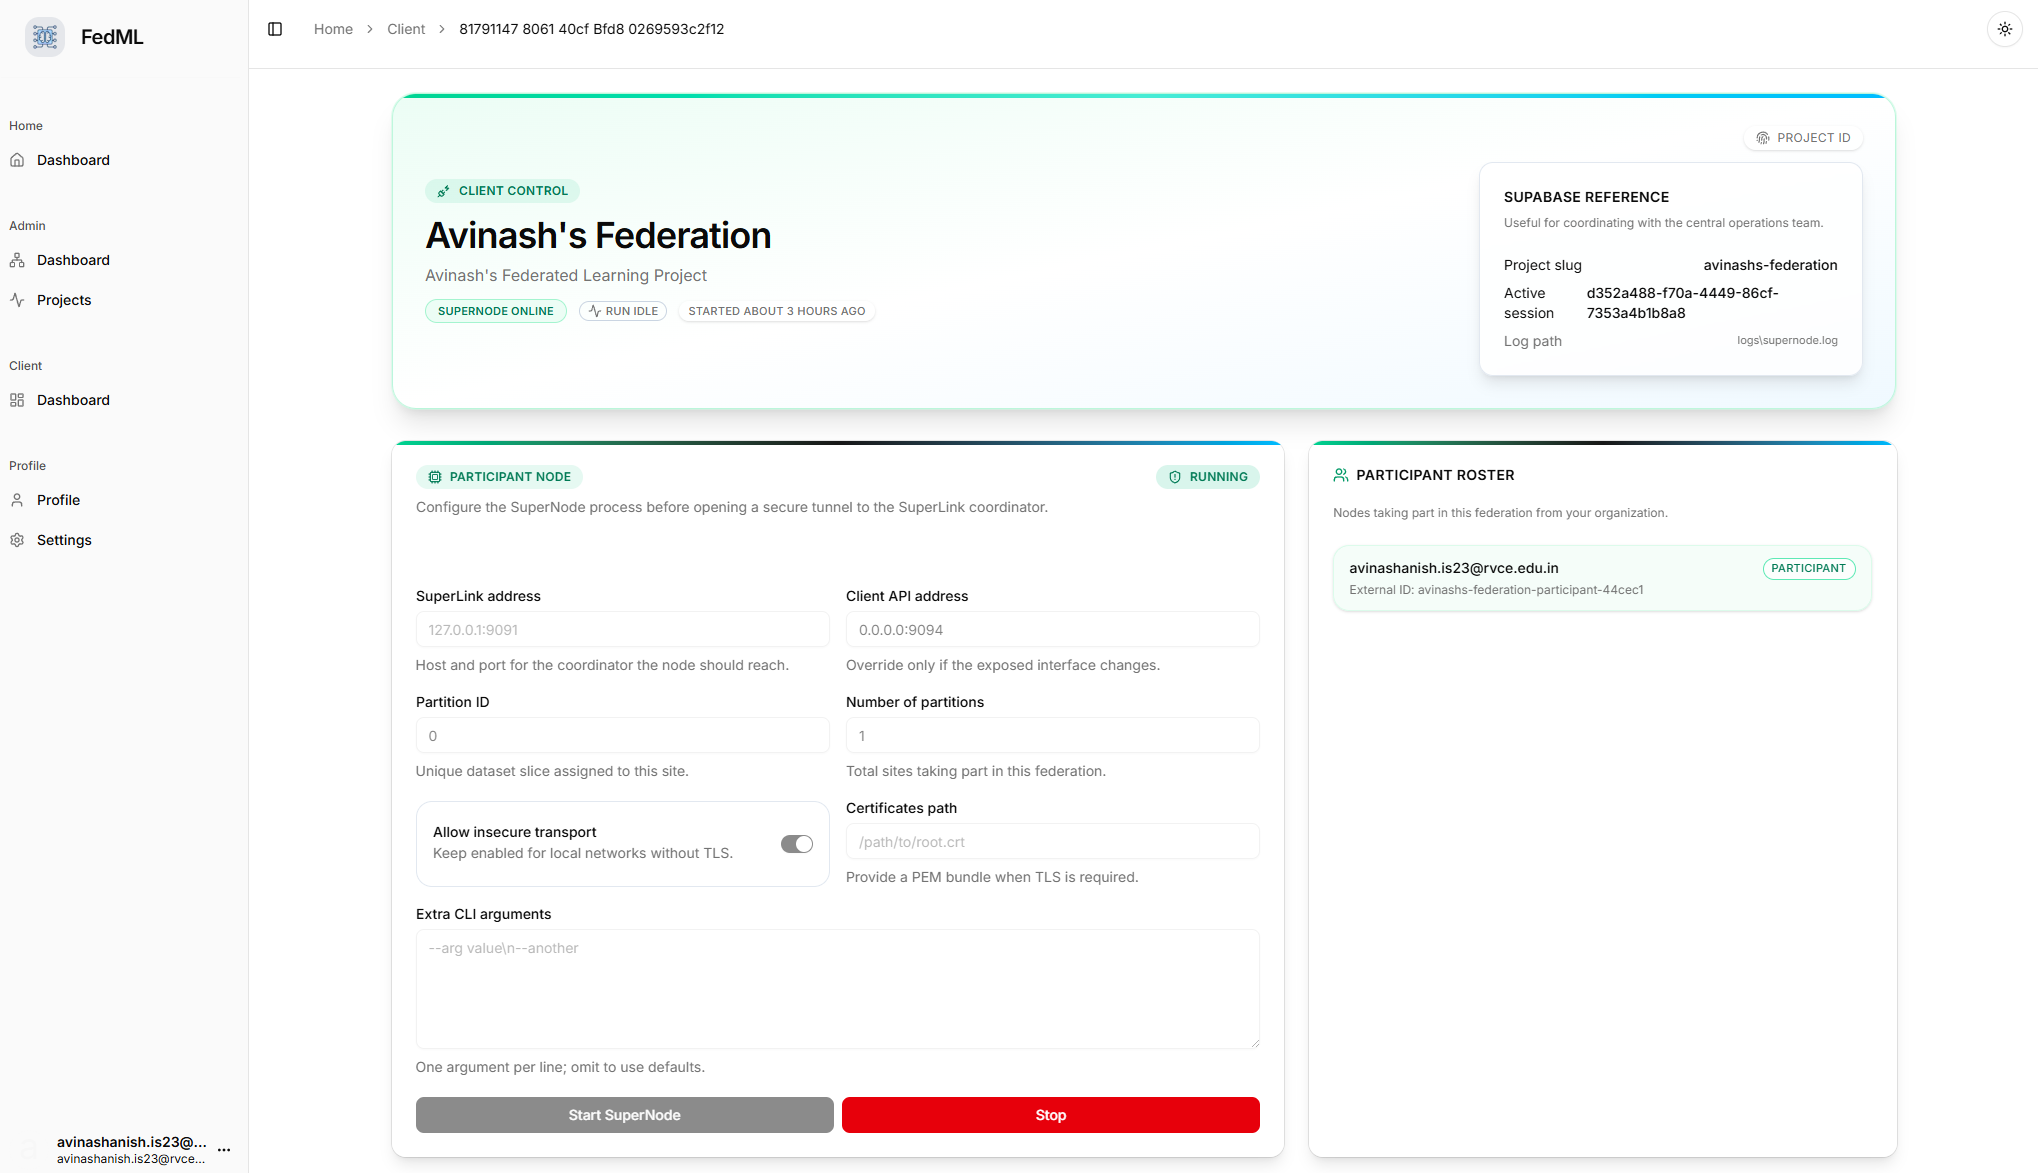
\includegraphics[width=0.9\textwidth]{images/screenshots/fedml-client-project-details.png}
    \caption{Hospital Client interface showing local training status and dataset statistics.}
    \label{fig:client_view}
\end{figure}

\section{Codebase and Setup}

This section provides comprehensive details regarding the project repository, local installation, and containerized deployment procedures.

\subsection{Repository and Version Control}

The project source code is hosted on GitHub and can be accessed or cloned using the following repository URL:

\begin{lstlisting}[language=bash]
# Repository URL
https://github.com/CubeStar1/federated-learning.git

# Cloning the repository
git clone https://github.com/CubeStar1/federated-learning.git
cd federated-learning
\end{lstlisting}

\subsection{Repository Architecture}

The system is modularized into several key components to ensure scalability and ease of deployment:

\begin{itemize}
    \item \textbf{admin-server/}: A FastAPI-based orchestration service that manages the central Flower SuperLink and training runs.
    \item \textbf{client-server/}: A FastAPI service designed for participant sites to manage local SuperNode instances.
    \item \textbf{flower-app/}: The core application containing the federated learning strategy, model definitions, and training loops.
    \item \textbf{frontend/}: A Next.js dashboard providing real-time metrics and administration capabilities.
    \item \textbf{db/}: Contains the Supabase SQL schema for persistent storage of metrics and logs.
\end{itemize}

\subsection{Local Development Setup}

\textbf{Backend Services Installation:}

To set up the backend environment, follow these steps to install the necessary Python dependencies:

\begin{lstlisting}[language=bash]
# Create and activate virtual environment
python -m venv .venv
.\.venv\Scripts\activate  # On Windows

# Install core and shared dependencies
pip install flwr
pip install -r requirements.txt

# Install the flower application in editable mode
cd flower-app
pip install -e .
\end{lstlisting}

\textbf{Frontend Dashboard Installation:}

The frontend requires Node.js and can be initialized as follows:

\begin{lstlisting}[language=bash]
cd frontend
npm install
npm run dev
\end{lstlisting}

\subsection{Docker Deployment}

The system supports containerized deployment for both the admin and client servers, simplifying the setup of the federated environment.

\textbf{Building Docker Images:}

\begin{lstlisting}[language=bash]
# Build Admin Server image
docker build -t fedml-admin -f admin-server/Dockerfile .

# Build Client Server image
docker build -t fedml-client -f client-server/Dockerfile .
\end{lstlisting}

\textbf{Running Containers:}

\begin{lstlisting}[language=bash]
# Start Admin Server container
docker run -p 8000:8000 --env-file .env fedml-admin
\end{lstlisting}

\subsection{Environment Configuration}

Create a \texttt{.env} file in the root directory to configure the services:

\begin{lstlisting}[language=bash]
SUPABASE_URL=https://your-project.supabase.co
SUPABASE_KEY=your-service-role-key
PROJECT_SLUG=fed-healthcare-project
\end{lstlisting}

\subsection{Windows-Specific Dependency Patch}

Due to process termination issues in the Flower library on Windows, modify line 56 of \texttt{venv\textbackslash Lib\textbackslash site-packages\textbackslash flwr\textbackslash supercore\textbackslash app\_utils.py}:

\begin{lstlisting}[language=Python]
# Original: os.kill(os.getpid(), signal.CTRL_C_EVENT)
# Patch:
os.kill(os.getpid(), signal.SIGTERM)
\end{lstlisting}

